% !TeX root = ./homework.tex
\section{题解3}
\subsection{问题a}
将坐标点按横坐标排序,选出左边的$\lfloor\frac{n}{2}\rfloor$个点为一部分,剩下的为第二部分。

\subsection{问题b}
\begin{figure}[htbp]
    \centering
    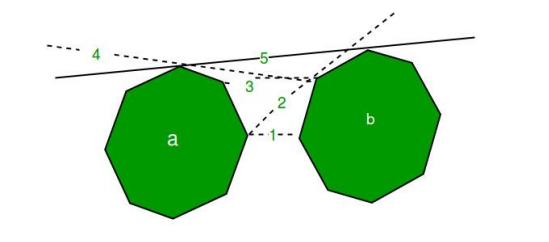
\includegraphics[width=1\textwidth]{截图.png}
    \caption{示意图}
\end{figure}
查找合并凸包的上方连线时,从左边部分的最右点和右边部分的最左点连线开始查找:
\begin{enumerate}
    \item 固定右边的点,遍历左凸包上在连线上方的点
    \item 找到与原连线夹角最大的新连线
    \item 固定左边的点,遍历右凸包上在连线上方的点
    \item 找到与原连线夹角最大的新连线
    \item 重复直到找不到新连线
\end{enumerate}
查找合并凸包的下方连线时,从左边部分的最右点和右边部分的最左点连线开始查找:
\begin{enumerate}
    \item 固定右边的点,遍历左凸包上在连线下方的点
    \item 找到与原连线夹角最大的新连线
    \item 固定左边的点,遍历右凸包上在连线下方的点
    \item 找到与原连线夹角最大的新连线
    \item 重复直到找不到新连线
\end{enumerate}

\subsection{问题c}
算法的主要时间都花在将小凸包合并为大凸包的过程上。